% Beijing National Day School General LaTex style 
% This is unofficial so you can modified it by yourself
% See https://bndsecon.com/ for more information in BNDS
% To be honest, this is my school project so it may be a little bit haste

% ------------------------------------------------------------------------------------------
% Features 1: You can modified the font size at here. I provide three font sizes: 10pt 11pt 12pt
% Remember! You need to comment the rest of the two options codes 
% \documentclass[10pt]{report}
% \documentclass[11pt]{report}

\documentclass[12pt]{report}
% ------------------------------------------------------------------------------------------
\usepackage{FORMAT}

\usepackage{fancyhdr}
\usepackage{graphicx}
\usepackage{tikz}
\usepackage{qrcode} % QR code generator 
\usepackage{gensymb}  % \degree
\usepackage{pgfornament}
\usepackage{eso-pic}
\usepackage{siunitx}
\usepackage{tikzrput}
\usepackage{tabularx}
\usepackage{fontspec}
\usepackage{longtable}
\usepackage{lipsum}
\usepackage{setspace}
\usepackage{hyperref}
\usepackage{amsmath}
\usepackage{esint}
\usepackage[autostyle, english = american]{csquotes}  % quote orientation
\DeclareGraphicsExtensions{.png,.pdf}
% ------------------------------------------------------------------------------------------
% Features 2: You can modified the page margins at here

\usepackage[top=1in,bottom=1in,left=1in,right=1in,xetex]{geometry}
% ------------------------------------------------------------------------------------------

% ------------------------------------------------------------------------------------------
% Features 3: You can modified the line spread at here. 
%             1 is default 
%             1.3 is pretty good
% \linespread{0.8}
% \linespread{1}
\linespread{1.3}
% \linespread{1.5}
% \linespread{2} 
% ------------------------------------------------------------------------------------------


% ------------------------------------------------------------------------------------------
% Features 3: Produce or don't produce a List of Tables page 

% \tablespagetrue 
\tablespagefalse

% ------------------------------------------------------------------------------------------


% ------------------------------------------------------------------------------------------
% Features 3: Produce or don't produce a List of Figures page 

% \figurespagetrue 
\figurespagefalse

% ------------------------------------------------------------------------------------------






% ------------------------------------------------------------------------------------------
% Features 4: You can modified the font at here, I give you a very elegant font 

% \setmainfont{texgyrepagella-regular.otf}[
% BoldFont = texgyrepagella-bold.otf ,
% ItalicFont = texgyrepagella-italic.otf ,
% BoldItalicFont = texgyrepagella-bolditalic.otf ]

% \setsansfont{texgyrepagella-regular.otf}[
% BoldFont = texgyrepagella-bold.otf ,
% ItalicFont = texgyrepagella-italic.otf ,
% BoldItalicFont = texgyrepagella-bolditalic.otf ]

% \setmonofont{texgyrepagella-regular.otf}[
% BoldFont = texgyrepagella-bold.otf ,
% ItalicFont = texgyrepagella-italic.otf ,
% BoldItalicFont = texgyrepagella-bolditalic.otf ]


% ------------------------------------------------------------------------------------------


% ------------------------------------------------------------------------------------------
% Features 5: I have carefully prepared the page decoration for you. You can check out more decorations on this official website  
% https://ctan.org/pkg/pgfornament


% \usetikzlibrary{positioning, arrows.meta, chains, scopes, calc}
% \newcommand\AtPageUpperRight[1]{\AtPageUpperLeft{%
% \put(\LenToUnit{\paperwidth},\LenToUnit{0\paperheight}){#1}%
%  }}%
% \newcommand\AtPageLowerRight[1]{\AtPageLowerLeft{%
% \put(\LenToUnit{\paperwidth},\LenToUnit{0\paperheight}){#1}%
% }}%
% \AddToShipoutPictureBG{%
%   \AtPageUpperLeft{\put(0,-25){\pgfornament[width=1.75cm]{39}}}
%   \AtPageUpperRight{\put(-50,-25){\pgfornament[width=1.75cm,symmetry=v]{39}}}
%   \AtPageLowerLeft{\put(0,25){\pgfornament[width=1.75cm,symmetry=h]{39}}}
%   \AtPageLowerRight{\put(-50,25){\pgfornament[width=1.75cm,symmetry=c]{39}}}
% }
%
% ------------------------------------------------------------------------------------------

\MakeOuterQuote{"}



% ------------------------------------------------------------------------------------------
% Features 6: I provide you a fancy head at here. You can change the name or the logo here

% \pagestyle{fancy}
% \fancyhf{}
% \fancyhead[L]{
% 	\begin{minipage}[c]{0.06\textwidth}
% 		
\includegraphics[height=7.5mm]{pic\BNDS_Logo_Horizon.png}
% 	\end{minipage}
% 	\begin{minipage}[c]{0.4\textwidth}
% 	You can write anything here.
% 	\end{minipage}}
% \fancyhead[R]{Your Title / Author name}




% ------------------------------------------------------------------------------------------


% ------------------------------------------------------------------------------------------
% Features 6: I provide you a fancy foot at here. You can change the name or the logo here


% \fancyfoot[L]{
% 	\begin{minipage}[c]{0.06\textwidth}
% 		
\includegraphics[height=7.5mm]{pic\BNDS_Logo_Small.png}
% 	\end{minipage}}
% \fancyfoot[R]{
% 	\begin{minipage}[c]{0.06\textwidth}
% 		
\includegraphics[height=7.5mm]{pic\BNDS_Logo_Small.png}
% 	\end{minipage}}
% \fancyfoot[C]{ \thepage }

% \pagestyle{fancy}

% ------------------------------------------------------------------------------------------


\DeclareGraphicsExtensions{.png,.pdf}

\begin{document}


\title{How to survive in\\
            BNDS}

\author{Your name}

\beforepreface
\prefacesection{Abstract}

Welcome to BNDS. This is my Abstract. 


Abstract is the most important part in your paper (From essay writting perspective).

So! Pay more attention to your writing. 
\prefacesection{Acknowledgements}

Thank Thank Thank Thank Thank. 
\afterpreface
\chapter{Introduction}

\section{Background Information}

You can provide background information here




\subsection{Background Research}

You can talk about background research here
\chapter{Big Chapter Title}


\chaptermark{Short Chapter Title}





\section{Introduction}
\lipsum[1-2]
\begin{equation}
    \frac{\left( {{1}\Bigg/{\sqrt{2\pi \sigma _{0}^{2}}}} \right) ^n\exp \left\{ {{\left( -\sum_{i=1}^n{\left( x_i-\mu _0 \right) ^2} \right)}\Bigg/{2\sigma _{0}^{2}}} \right\}}{\left\{ {{1}\Bigg/{\left( \frac{2\pi}{n} \right) \sum_{i=1}^n{\left( x_i-\mu _0 \right) ^2}}} \right\} ^{\frac{n}{2}}e^{-\frac{n}{2}}}
\end{equation}


\section{Automatic A+ Maker Model}

\lipsum[1-2]
\begin{figure}
    \centering
    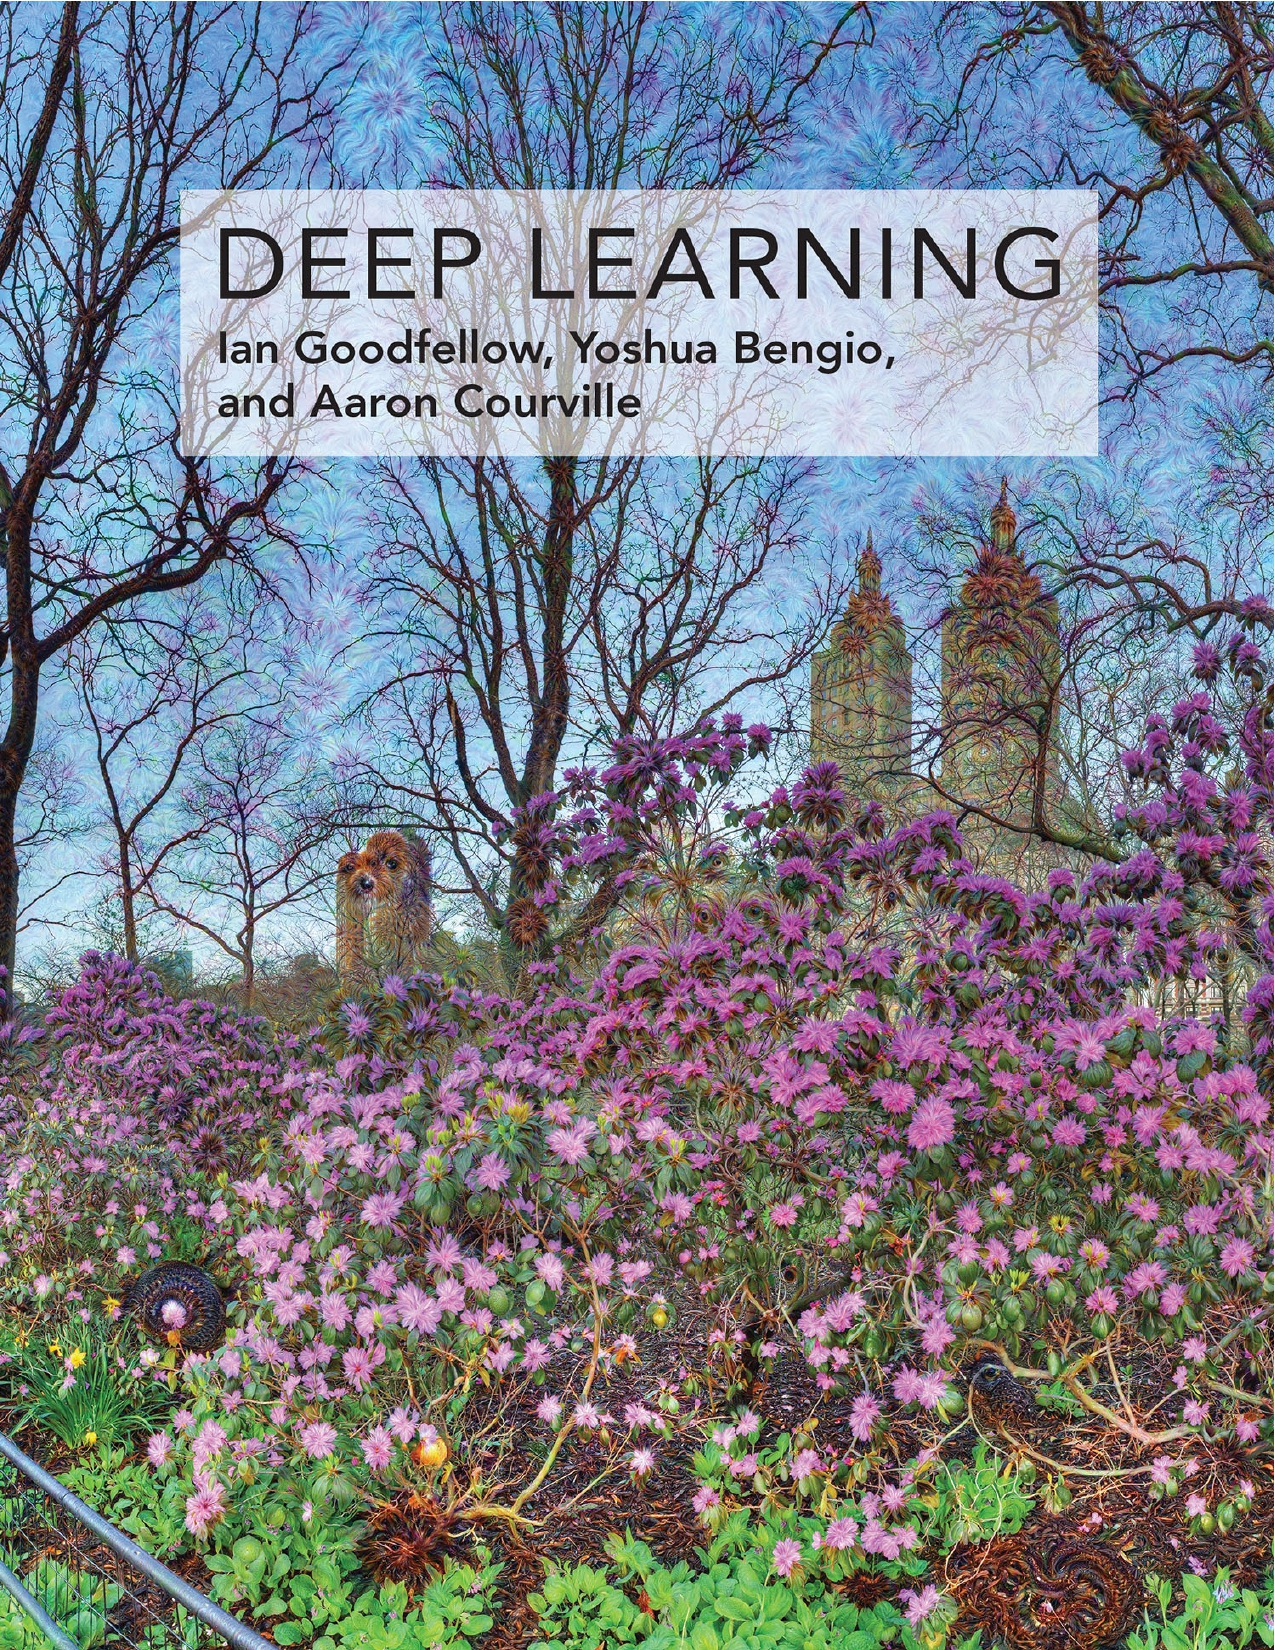
\includegraphics[width=8cm]{pic/DeepLearning.jpg}
\end{figure}
\lipsum[1-2]

\begin{equation}
    \left\{ \begin{array}{l}
        \nabla \cdot \boldsymbol{E}=\frac{\rho}{\varepsilon _0}\\
        \nabla \times \boldsymbol{E}=-\frac{\partial \boldsymbol{B}}{\partial t}\\
        \nabla \cdot \boldsymbol{B}=0\\
        c^2\nabla \times \boldsymbol{B}=\frac{\boldsymbol{j}}{\varepsilon _0}+\frac{\partial \boldsymbol{E}}{\partial t}c^2\\
    \end{array} \right. 
\end{equation}



\begin{equation}
    \left\{ \begin{array}{l}
        \oiint_{\partial \Omega}{\boldsymbol{E}\cdot \mathrm{d}s}=\frac{Q}{\varepsilon _0}\\
        \oiint_{\partial \Omega}{\boldsymbol{B}\cdot \mathrm{d}s}=0\\
        \oint_{\partial \Omega}{\boldsymbol{E}\cdot \mathrm{d}\ell}=-\frac{\mathrm{d}\varPhi _B}{\mathrm{d}t}\\
        \oint_{\partial \Sigma}{\boldsymbol{B}\cdot \mathrm{d}\ell}=\mu _0I+\mu _0\varepsilon _0\frac{\mathrm{d}\varPhi _E}{\mathrm{d}t}\\
    \end{array} \right.
\end{equation}



\subsection{Super humam practice finisher}

\lipsum[1-2]

\section{Conclusions}
\lipsum[1-5]
This is the conclusion part of the paper body. 
\chapter{Concluding Remarks}

According to our research, ...



% ------------------------------------------------------------------------------------------
% Features 6: I have carefully prepared the page decoration for you. You can check out more decorations on this official website  


% uncomment this section for a Appendix insertion
% \appendix
% \chapter{Appendix}

% ------------------------------------------------------------------------------------------



\bibliographystyle{unsrt}


% ------------------------------------------------------------------------------------------
% Features 7: You can easily manage your reference here


\bibliography{bibEG}

% ------------------------------------------------------------------------------------------





\end{document}
